%%=============================================================================
%% Methodologie
%%=============================================================================

\chapter{Methodologie}
\label{ch:methodologie}

%% TODO: Hoe ben je te werk gegaan? Verdeel je onderzoek in grote fasen, en
%% licht in elke fase toe welke stappen je gevolgd hebt. Verantwoord waarom je
%% op deze manier te werk gegaan bent. Je moet kunnen aantonen dat je de best
%% mogelijke manier toegepast hebt om een antwoord te vinden op de
%% onderzoeksvraag.

% \lipsum[21-25]

\begin{figure}
	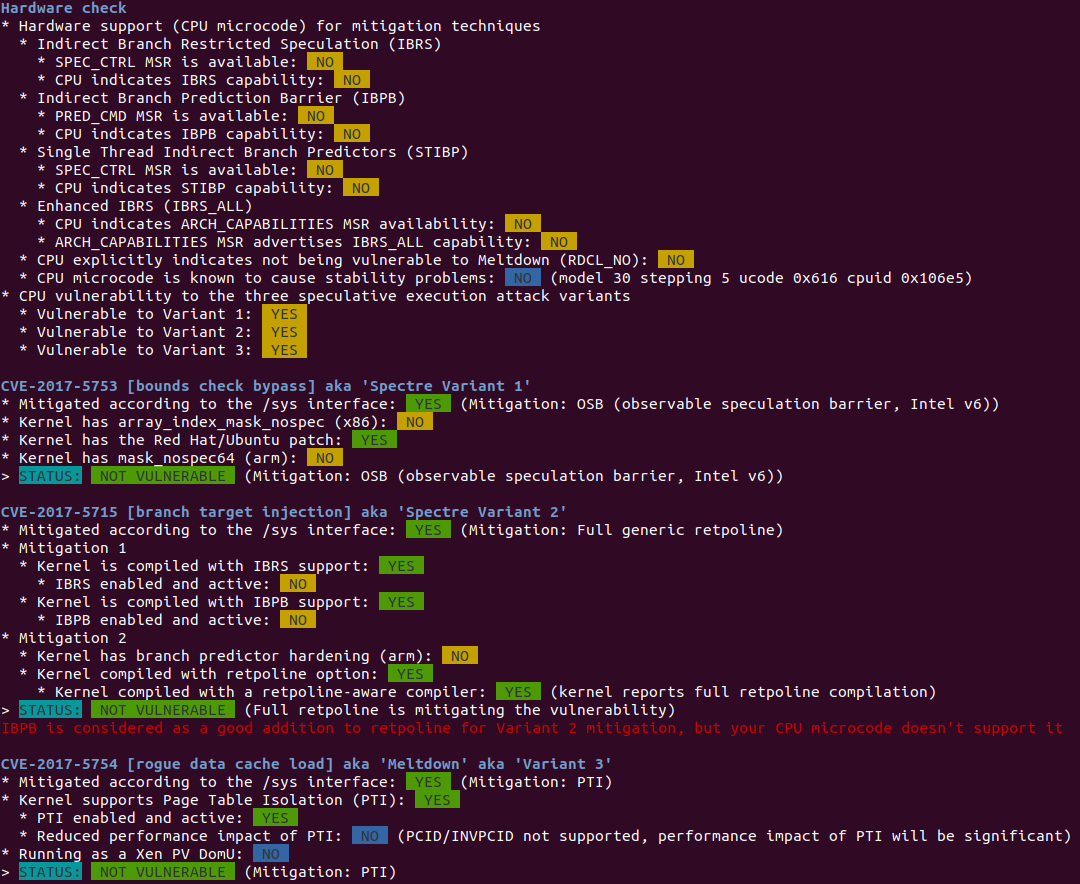
\includegraphics[width=1.0\linewidth]{img/checker_patched.png}
	\caption{Kwetsbaarheid checken beveiligd systeem}
	\label{fig:checker_patched}
\end{figure}

\begin{figure}
	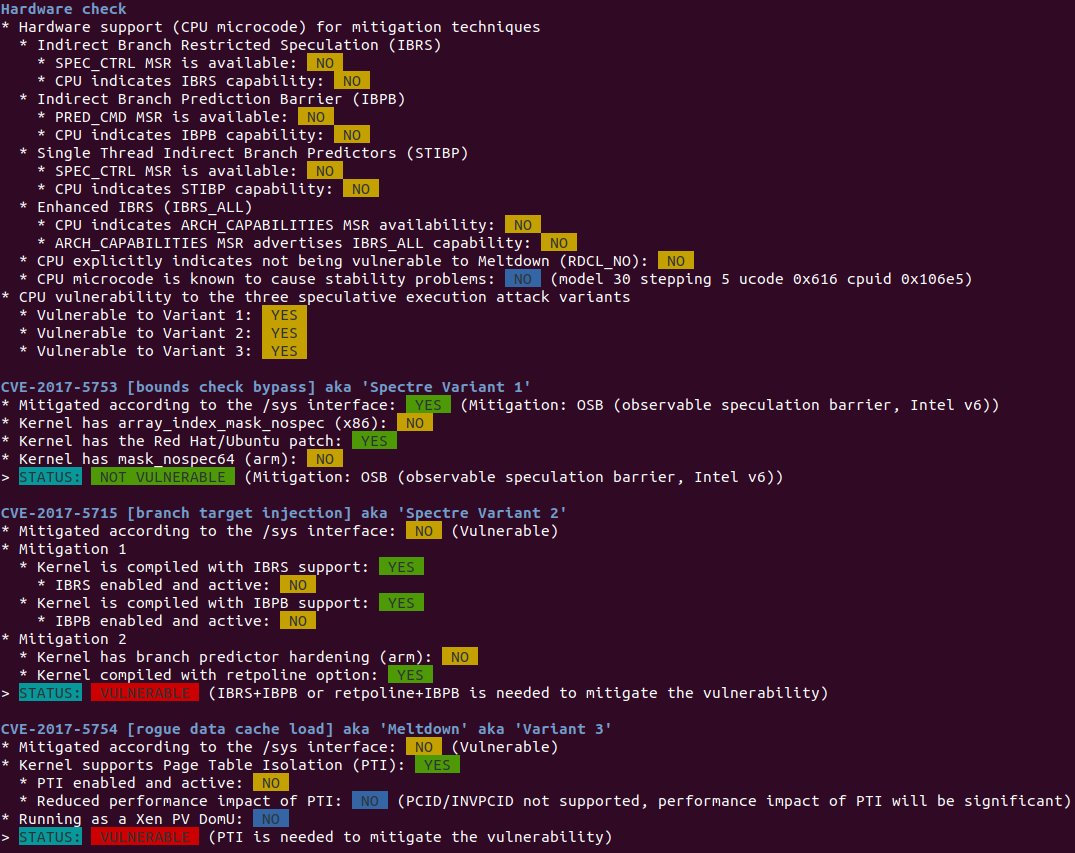
\includegraphics[width=1.0\linewidth]{img/checker_vulnerable.png}
	\caption{Kwetsbaarheid checken kwetsbaar systeem}
	\label{fig:checker_vulnerable}
\end{figure}

\begin{figure}
	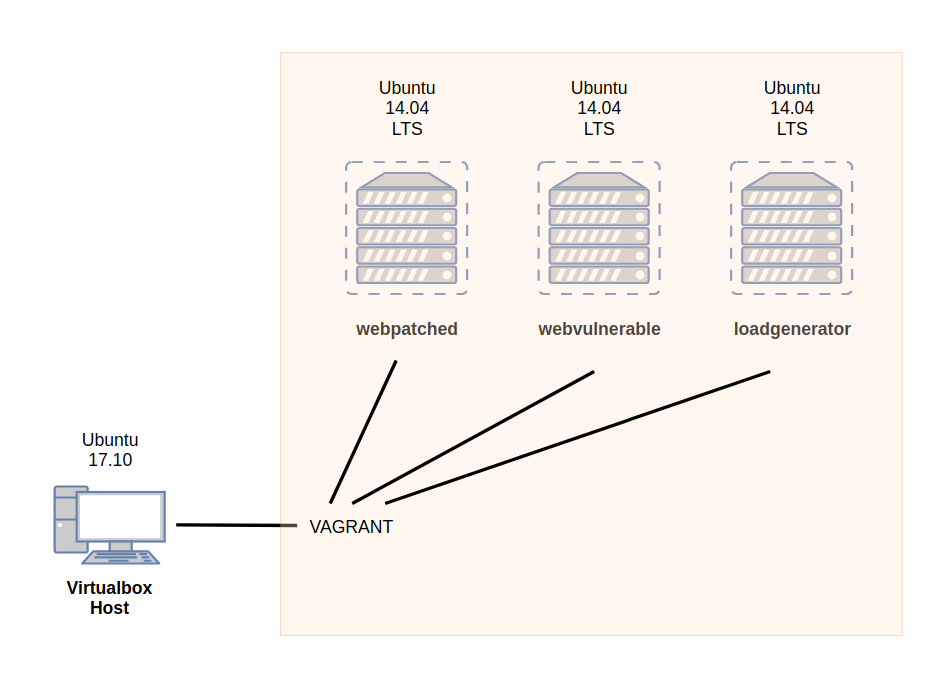
\includegraphics[width=1.0\linewidth]{img/testopstelling.png}
	\caption{testopstelling}
	\label{fig:testopstelling}
\end{figure}

Voor de uitwerking van deze scriptie werd eerst de testopstelling (figuur \ref{fig:testopstelling}) opgezet.
Dit is gedaan met behulp van Vagrant.

Er werd gekozen voor Vagrant omdat dit een snelle en reproduceerbare manier is om meerdere virtuele machines op te zetten. Om de servers te configureren werd Ansible gebruikt.

\section{Opstelling}
De volledige setup is gedefinieerd in één file: de Vagrantfile.
In de Vagrantfile zijn er drie virtuele machines gedefinieerd. Twee ervan zijn webservers: één kwetsbaar voor Meltdown en Spectre, en één met de patches. De andere is een client die de belasting genereert. De tools die gebruikt worden voor belasting te genereren zijn 'autobench', 'ab' en 'redis-benchmark'. Het besturingssysteem is Ubuntu 14.04 64-bits. Dit besturingssysteem zit in de trusty64 Vagrant box. De drie virtuele machines kregen elk 4 CPU's toegewezen. Het hostsysteem heeft 4 fysieke en 8 virtuele kernen. Om geen bottleneck te creëren worden het aantal toegewezen CPU's gelijkgesteld met het aantal fysieke CPU's van het hostsysteem. Meer dan 4 zou waarschijnlijk de prestaties van de virtuele machine verminderen.

Er werd gekozen voor deze box omdat het regelmatig geüpdatet wordt en door Canonical zelf wordt onderhouden.
De virtuele machine provider is virtualbox. Provisioning wordt voorzien door Ansible en is in Vagrant geconfigureerd.

\section{Patches}
Standaard zijn de patches geïnstalleerd, het is dus een kwestie van ze uit te schakelen voor de kwetsbare server.
Dit wordt gedaan via kernel parameters (\textit{spectre\_v2=off} en \textit{nopti}). Er worden items toegevoegd aan het einde van de 'grub kernel' opdrachtregel voor zowel normale als herstelmodi.
Alleen de patches voor variant 2 en variant 3 (Meltdown) zijn uitgeschakeld (figuur \ref{fig:checker_patched} en \ref{fig:checker_vulnerable}) omdat variant 1 geen meetbare impact heeft \parencite{Redhat2018a}.